\documentclass{standalone}



\usepackage{graphics}
\usepackage{color}
\usepackage{tikz}

\definecolor{blue}{RGB}{0, 114, 189}
\definecolor{red}{RGB}{212.5000,81.2500,   24.5000}
\definecolor{yellow}{RGB}{232.2500, 173.5000,   31.2500}
\definecolor{violet}{RGB}{123.5000,  46.0000, 139.0000}
\definecolor{green}{RGB}{116.5000, 168.5000,  47.0000}


\begin{document}
 \begin{figure}[h]
 \centering
  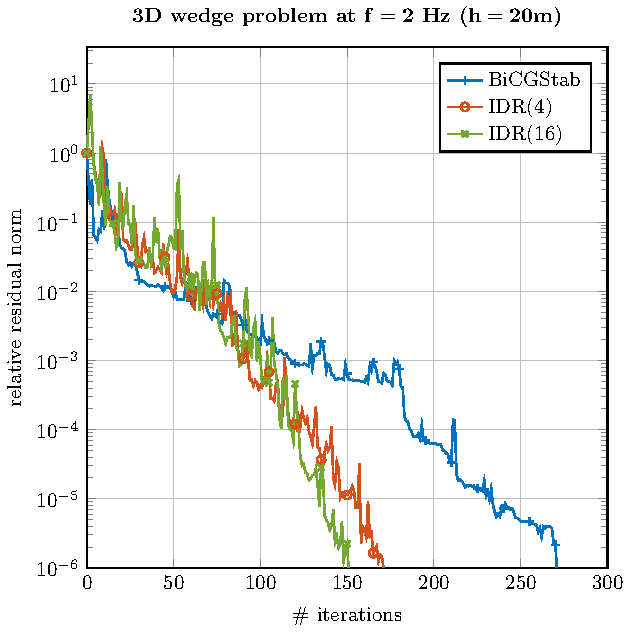
\includegraphics{wedge3d_f2_new3.pdf}
 \end{figure}
 
 \begin{tikzpicture}[overlay]
%   \draw[color=blue, thick] (-4.3,3.23) -- (-4.3,2.25) -- (-2.85,2.25) --cycle;
  \draw[color=blue, thick, dashed] (-4.3,3.23) -- (-4.3,2.05) -- (-2.56,2.05) --cycle;
  \node[color=blue, rotate=-34] at (-3.6,2.55) {\texttt{-1.7e-2}};
   
  \draw[color=red, thick, dashed] (-8.05,5.7) -- (-8.05,3.92) -- (-6.6,3.92) --cycle;
  \node[color=red, rotate=-49] at (-7.5,4.7) {\texttt{-3.1e-2}};
  
  \draw[color=green, thick, dashed] (-6.85,3.51) -- (-6.85,1.5) -- (-5.4,1.5) --cycle;
  \node[color=green, rotate=-54] at (-6.2,2.3) {\texttt{-3.5e-2}};
 \end{tikzpicture}

 
\end{document}
